\documentclass[paper=a4paper,jafontsize=9pt,head_space=15mm,gutter=20mm,
twocolumn,number_of_lines=49, line_length=26zw]{myuarticle}

\begin{document}

\title{{\Large\bfseries\gtfamily 環境情報のセンシングを用いた他者の環境評価を表現するロボットシステム}}
\author{\\\ 22120165 中村龍造 \\ (指導教員 : 佐藤宏樹)\\ \\}
\date{}
\maketitle

\section{はじめに}
生活空間には,人間以外にも多くの存在が共存している.それらの存在は,それぞれ独自の感覚や基準で環境を捉えているが,その感覚を直接共有することはできない.このような「他者」の経験を理解し,共感することは,多様な存在との共生を考える上で重要な課題となっている.

本稿では,取得した環境データに対して,人間,動植物,非生物などといった複数の他者からの評価基準を設定し,評価結果をロボットの身体的動作を通して表現するシステム(以下「本システム」)を提案する.本システムを通じて,ユーザーが他者にとっての快適さを知り,他者への理解,関心を深めることで,多様な存在との対話の機会創出を目指す.

\section{関連研究と課題}

他者視点の表現に関する取り組みとしては,In the Eyes of the Animal\cite{Dezeen-2015-MarshmallowLaserFeastsEyes}のようなVRによる体験の共有や,rapoptosis\cite{--ソンヨン}のようなモノの自立的な意思決定の表現が提案されている.しかしこれらの手法は一時的な体験や特定の対象に限定されており,生活空間で継続的に他者視点の理解を促すことは難しい.
人間を対象とした場合でも,環境への評価は個々人で差異があり,客観的指標による評価のみならず,主観での評価を取り入れる必要がある\cite{Coulby-2020-ScopingReviewTechnologicalApproaches}.

\section{システム要件}

上記の課題を踏まえ,本研究では人間,動植物,非生物など,様々な他者を基準に,それらから見た環境の快・不快をロボットの身体的動作で表現するシステムを開発する.ロボットという物理的な存在を用いることで,生活空間における他者の視点を継続的に表現し,共生への理解を深めることを目指す.本システムの開発にあたって以下の3点を要件とする:

\begin{description}
  \item[継続的な表現:] 生活空間において,ロボットが常に存在し続けることで,環境変化に応じた他者の評価を途切れることなく表現できること
  \item[多様な他者の表現:] 人間,動植物,非生物など様々な他者の環境評価基準を設定し,それぞれの特徴を反映した動作で表現できること
  \item[日常的な理解支援:] ユーザーが特別な操作をすることなく,生活空間における他者との環境認識の違いを自然に理解できること
\end{description}

\subsection{全体のフロー}
本システムは,ユーザー,環境,センサー,ロボット,本システムの5つからなる.システム全体のフローを図\ref{fig:system-flow}に示す.
はじめに本システムが,センサーを通じて生活空間の環境データを取得する.他者を基準とした評価,評価に応じて快・不快をアピールするなどの行動命令を現実空間のロボットに送信する.ロボットは行動命令に従って人間にアピールする.それを見た人間が環境や他者に対して働きかけることで,他者にとってより快適な環境を得る.

\fboxsep=0pt            %画像と枠線をくっつける.
\fboxrule=1pt            %枠線の太さを1ptにする.
\begin{figure}[h]
  \centering
  \fbox{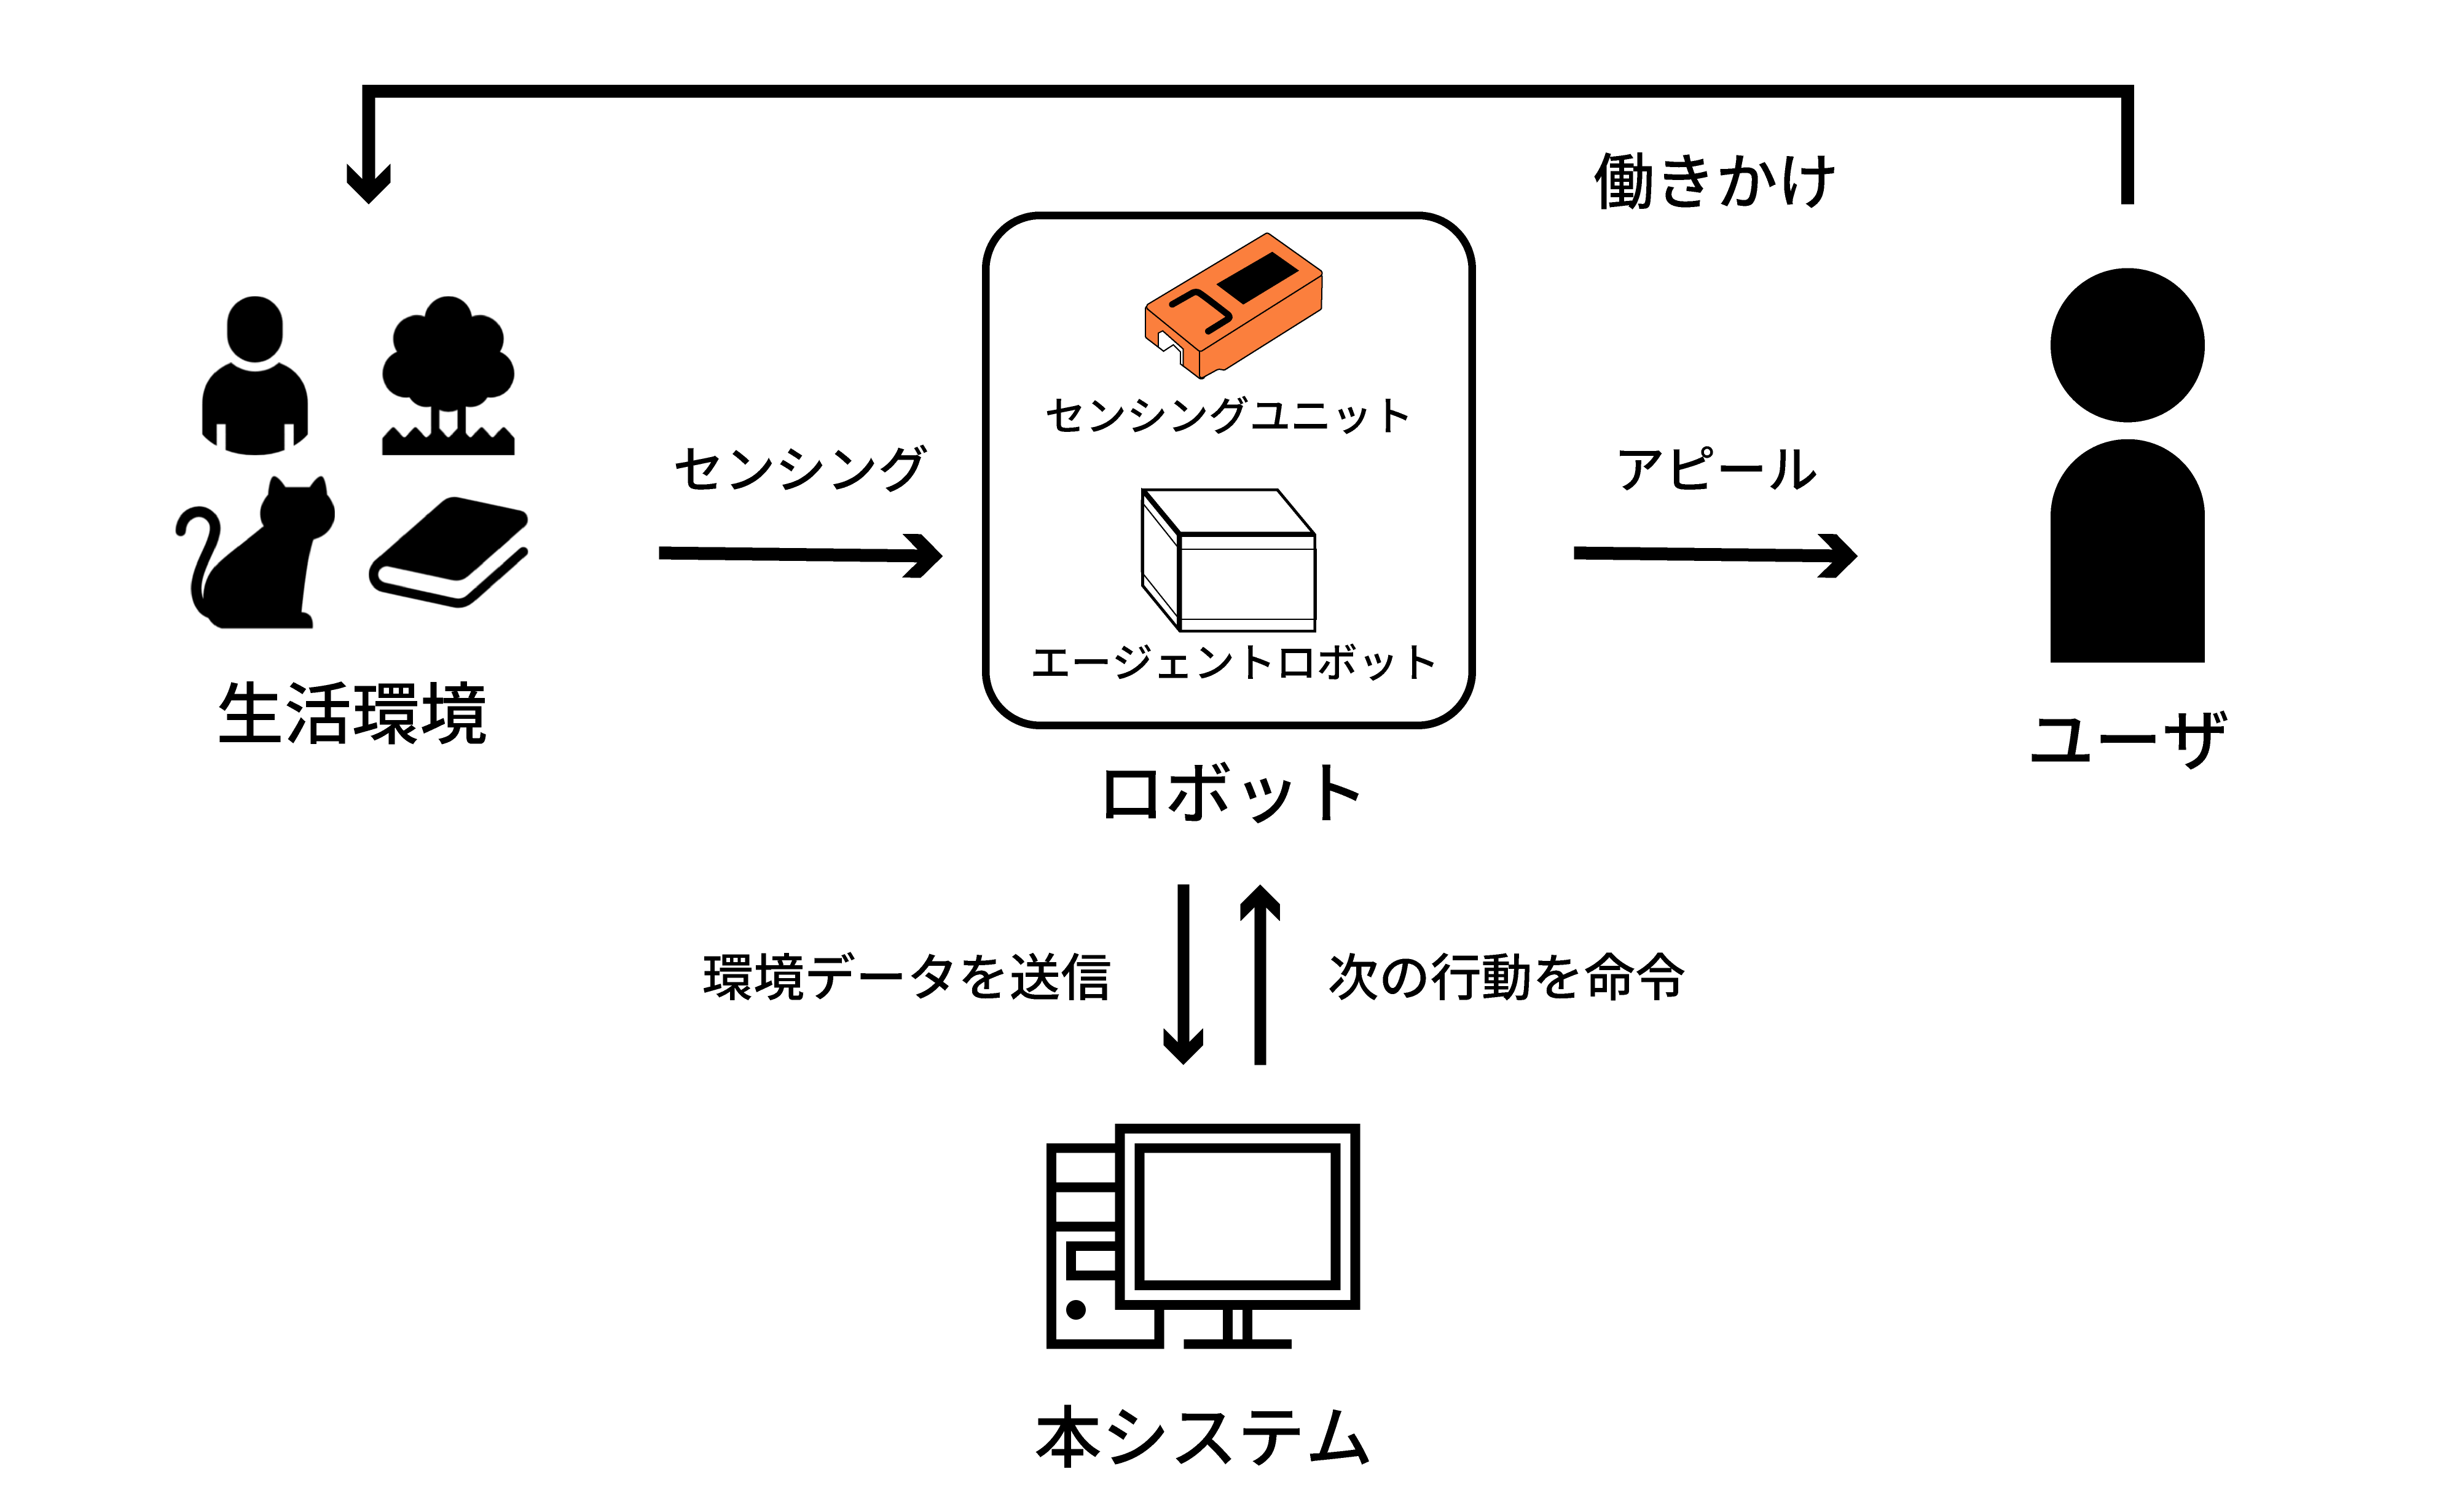
\includegraphics[keepaspectratio, clip,
  width=0.8\columnwidth]{resources/system_flow.png}}
  \caption{システム全体のフロー図}
  \label{fig:system-flow}
\end{figure}

\section{本システムの実装}
本システムは,センシングシステム,評価システム,アクション生成システム,ロボット制御システムから構成される.ハードウェアは,センシングデバイスにM5StickC(M5Stack社)を,ロボットにtoio(SONY社)を用いた.

本システムでは,各主体(人間,動物,物体など)について,その対象にとって最適な環境条件を設定し,現在の環境がその条件からどの程度離れているかに応じてロボットの動作を変化させる.
これらの条件に基づき,環境センサーから得られた測定値と最適条件との差異を評価し,ロボットの動作を決定する.
本システムの構造を図\ref{fig:system-structure}に示す.

\setcounter{figure}{2}
\begin{figure*}[t]
  \centering
  \begin{tabular}{ccc}
    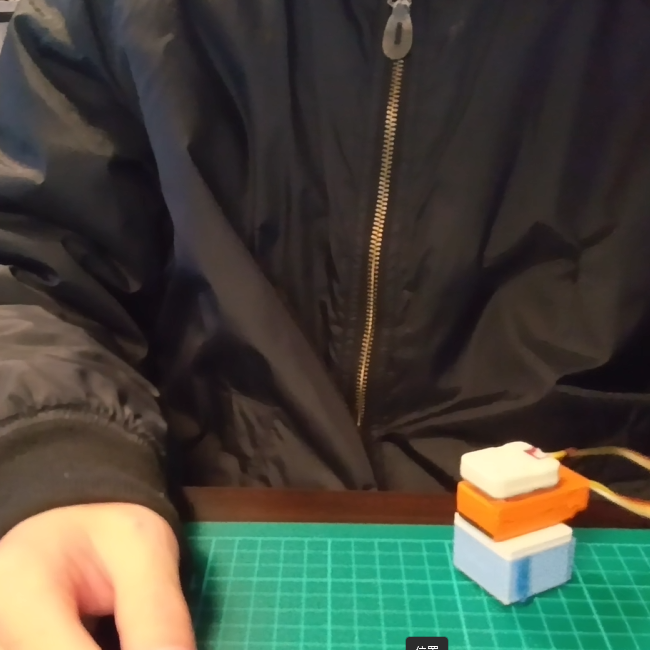
\includegraphics[width=0.25\textwidth]{resources/human.png} &
    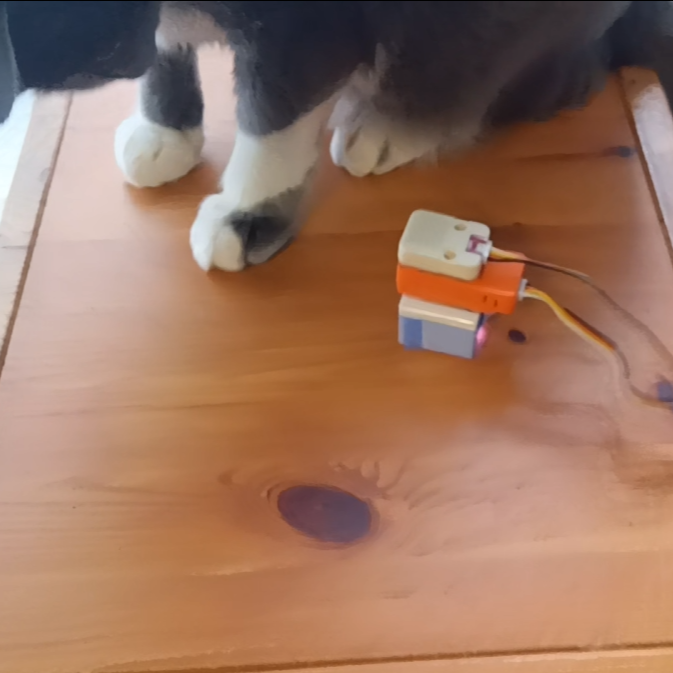
\includegraphics[width=0.25\textwidth]{resources/cat.png} &
    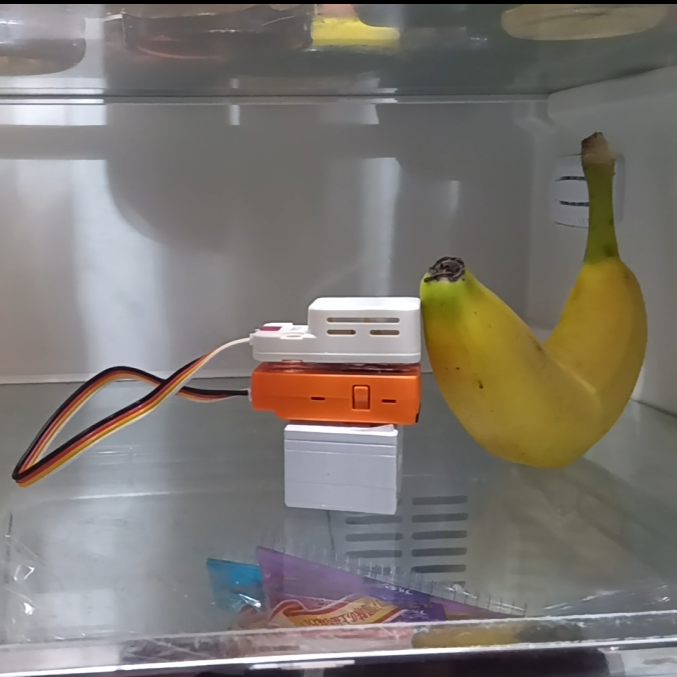
\includegraphics[width=0.25\textwidth]{resources/banana.png} \\
    人間の気温評価 & 猫の気温評価 & バナナの保存環境評価
  \end{tabular}
  \caption{システム動作検証の様子}
  \label{fig:system-test}
\end{figure*}

\setcounter{figure}{1}
\fboxsep=0pt            %画像と枠線をくっつける.
\fboxrule=1pt            %枠線の太さを1ptにする.
\begin{figure}[h]
  \centering
  \fbox{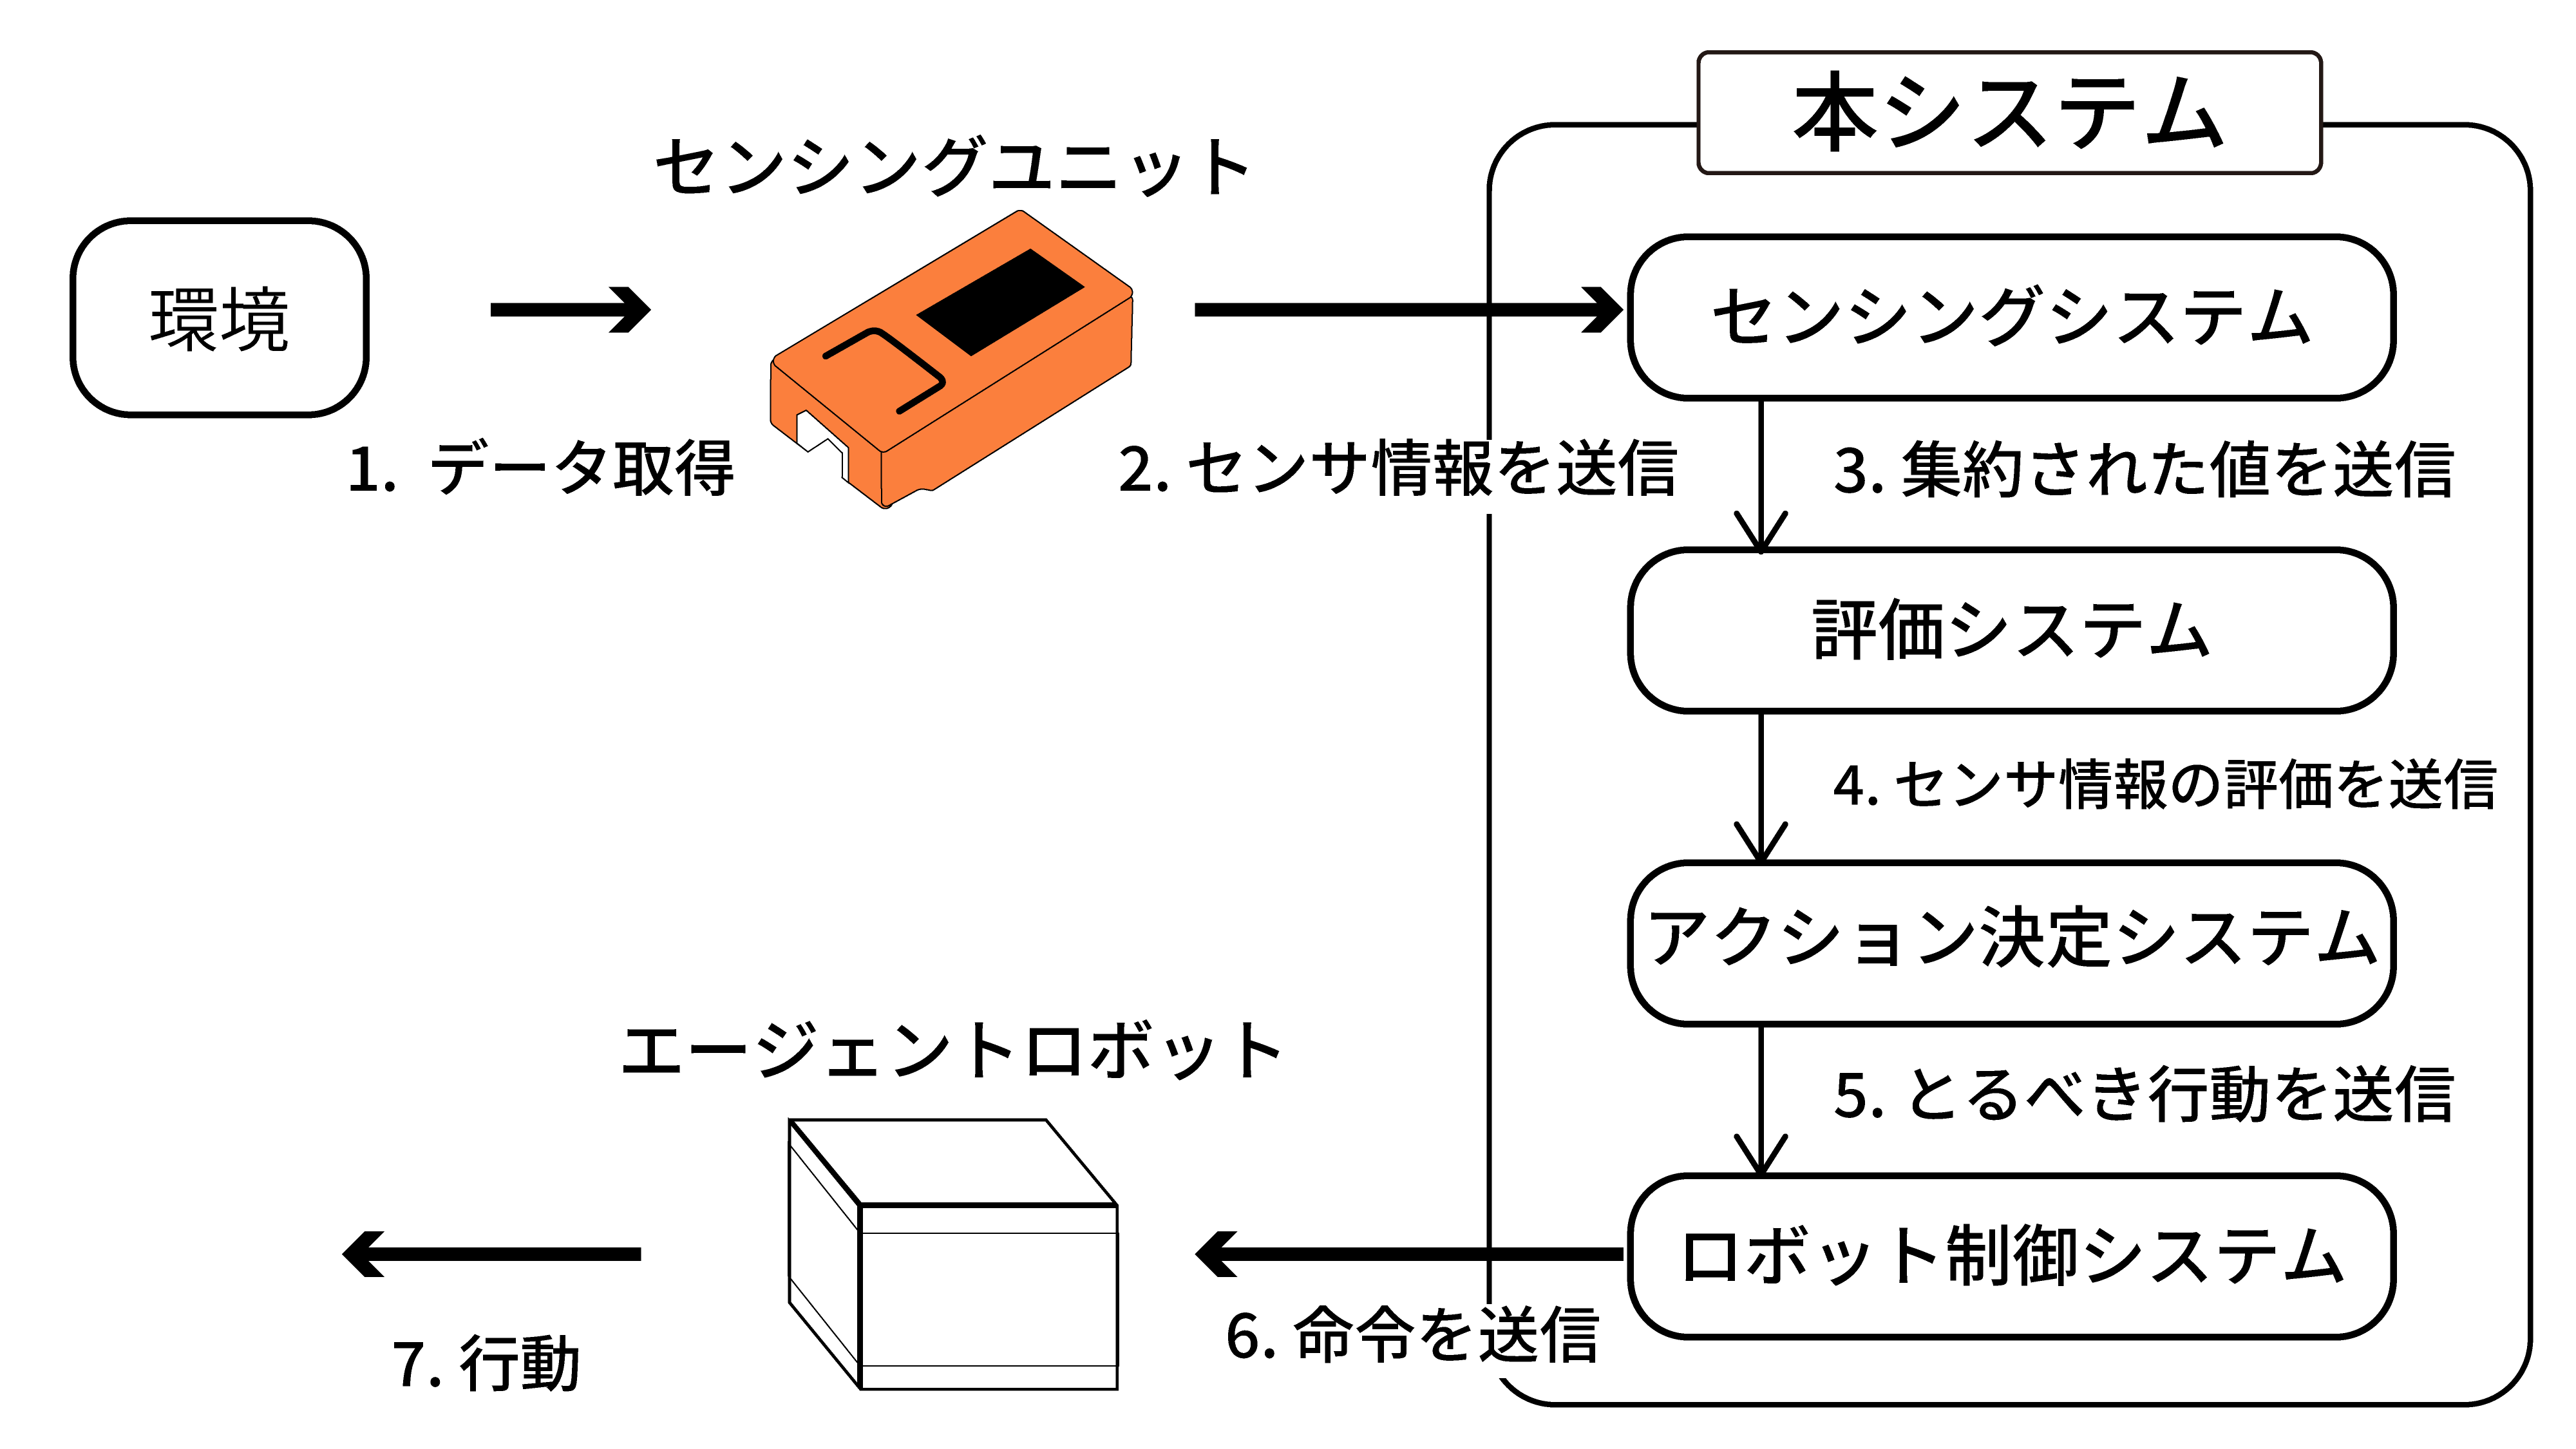
\includegraphics[keepaspectratio, clip,
  width=0.8\columnwidth]{resources/system_structure.png}}
  \caption{本システムの構造図}
  \label{fig:system-structure}
\end{figure}

\subsection{センシングシステムと評価システム}
センシングシステムは,センサーから送信されたデータを受け取り,以後のシステムにデータを提供する.
%\subsection{評価システム}
評価システムでは,センサーシステムから環境データを取得・評価し,評価データを生成する.評価データは,環境データと評価基準値との差をスコアとして所持している.対象データの評価では,例えば人間に適した気温であれば18~24℃などと,あらかじめ対象データの主体にとって最適な範囲を設定する.現在の気温が最適範囲から外れた場合,上回れば正の,下回れば負のスコアをもった評価データを生成する.システム開発者は評価主体とその評価対象ごとに,個別の評価システムを実装する必要がある.

\subsection{アクション生成システム}
アクション生成システムでは,評価システムから取得した評価データをもとに,評価に応じたアクション命令をロボット制御システムへ送る.アクション開発者は,主体および対象の環境データごとにアクションを作成しておく必要がある.本システムのアクションは,岡田ら\cite{岡田-2017-弱いロボ}の「弱いロボット」の概念を取り入れてデザインした.
%「弱いロボット」は,人間の介入や支援を引き出す手法として「よたよた」とした動きを用いている.本システムでも,この考え方に基づき,
環境が快適でない場合のアクションとして,直線的に移動せず,わずかに蛇行しながら進んだり,時折立ち止まったりする動きを実装した.このような不安定な動きによって,ロボットが困っているような印象を与え,ユーザーが環境を確認し,調整するきっかけとなることを期待している.

%アクションは「コマンド」のキューで構成される.コマンドはロボット動作用のより低レベルな命令と,動作の所要時間を所持しており,一連のコマンドを実行することで,1つの意味あるアクションを表現する.

%\subsection{ロボット制御システム}
%ロボット制御システムでは,実機toioとシステム上のtoioを識別するためのデータ管理および,アクション生成システムから取得したアクションの実行を行う.

\section{システムの動作検証}
本システムによってロボットが動作している様子を図\ref{fig:system-test}に示す.

本システムの動作検証では,人間,猫,バナナの3つを評価主体として動作検証を行った.

人間を評価主体とした場合,気温18~28℃\cite{JianZhuWuHuanJingWeiShengGuanLiJiZhunnituite|HouShengLaoDongSheng}を最適環境条件とし,快適時には直線的な移動,不快時には蛇行移動や激しい移動によってアピールを行う.

猫については,気温30~38℃\cite{stellaEnvironmentalAspectsDomestic2016}を最適環境条件とし,快適時はじっとして動かず,不快時には不規則な軌道や頻繁な方向転換で表現する.

バナナについては,気温14~20℃\cite{--バナナの},湿度45~85\%\cite{--JISZ87031983試験}を最適環境条件とし,快適時は定点でのゆっくりな回転,不快時にはランダムな往復運動を行う.これらの動作パターンは,環境条件からの逸脱度に応じて変化する.

本システムの動作検証を通じて,以下の課題が明らかになった.第一に,人間を評価主体とする場合,個人差や状況による快適条件の変動に対応する必要がある.そのため,ユーザーがリアルタイムに評価基準を調整できるインターフェースの実装が求められる.

第二に,猫などの移動する主体の評価において,センシング位置と主体の位置の不一致という問題が生じた.主体の追跡は技術的に困難であるため,温度や湿度など,空間的な変化が緩やかな環境要因を中心に評価を行い,人間の近傍でアピールする方式への変更を検討する必要がある.

第三に,バナナなどの生鮮品を評価対象とする場合,追熟過程による最適保存条件の変化に対応できていないことが判明した.この課題に対しては,現在のような即時的な評価だけでなく,環境データの長期的な記録と分析機能を実装し,対象の状態変化に応じた評価基準の調整が必要である.

\section{まとめと今後の展望}%{システムの制約と展望}
%本システムは,Bluetooth通信を用いているため,屋内での使用を前提とし,通信可能な範囲内での動作に限られる.また,評価対象は基準が明確で計測可能なものに限定される.
今後の展開として,ロボット間の協調動作の実装や,より正確な環境評価のためのセンシング手法の改善が考えられる.さらに,異なるセンサーやロボットを組み合わせることで,新たなユーザー体験の創出も期待できる.\\

%\section{おわりに}
%本研究では,環境データを他者の視点から評価し,ロボットの身体的動作を通じて表現するシステムを開発した.M5StickCとtoioを用いたプロトタイプシステムの実装により,他者にとっての快・不快を直感的に理解できるインタフェースを実現した.特に,『弱いロボット』の概念を取り入れることで,ユーザーを自然にシステムフローに組み込むことができた.

%今後は,より多様な他者の表現や,ロボット同士の協調動作の実装など,システムの拡張を進めていく.

%  ----- 参考文献 -----
% 参考文献リストの「参考文献」のスタイル
\renewcommand{\refname}{\normalsize 7.  参考文献}
{
  \footnotesize
  \bibliography{ref}
}
\bibliographystyle{junsrt}
\end{document}
